\documentclass[12pt, titlepage]{article}

\usepackage{fullpage}
\usepackage[round]{natbib}
\usepackage{multirow}
\usepackage{booktabs}
\usepackage{tabularx}
\usepackage{graphicx}
\usepackage{float}
\usepackage{hyperref}
\hypersetup{
    colorlinks,
    citecolor=black,
    filecolor=black,
    linkcolor=red,
    urlcolor=blue
}
\usepackage[round]{natbib}

\newcounter{acnum}
\newcommand{\actheacnum}{AC\theacnum}
\newcommand{\acref}[1]{AC\ref{#1}}

\newcounter{ucnum}
\newcommand{\uctheucnum}{UC\theucnum}
\newcommand{\uref}[1]{UC\ref{#1}}

\newcounter{mnum}
\newcommand{\mthemnum}{M\themnum}
\newcommand{\mref}[1]{M\ref{#1}}

\title{SE 3XA3: Software Requirements Specification\\Title of Project}

\author{Team \#1, Team Name
		\\ Anjola Adewale and adewaa1
		\\ Sheridan Fong and fongs7
		\\ Chelsea Maramot and maramotc
}

\date{\today}

% \input{../../Comments}

\begin{document}

\maketitle

\pagenumbering{roman}
\tableofcontents
\listoftables
\listoffigures

\begin{table}[H]
\caption{\bf Revision History}
\begin{tabularx}{\textwidth}{p{3cm}p{2cm}X}
\toprule {\bf Date} & {\bf Author} & {\bf Notes}\\
\midrule
3/14/22 & Chelsea & v1.0 Introduction \\

3/14/22 & All & v2.0 Anticipated and Unlikely Changes \\
3/14/22 & All & v3.0 Module Hierarchy \\
3/16/22 & Sheridan + Chelsea & v3.1 Module Hierarchy editing \\
3/16/22 & All & v4.0 Module Decomposition \\
3/16/22 & Chelsea & v5.0 Traceability Matrix \\
3/16/22 & Chelsea & v6.0 Use Hierarchy \\
3/18/22 & All & v7.0 Editing document \\
\bottomrule
\end{tabularx}
\end{table}

\newpage

\pagenumbering{arabic}

\section{Introduction}

Decomposing a system into modules is a commonly accepted approach to developing
software.  A module is a work assignment for a programmer or programming
team~ Parnas et al. (1984).  We advocate a decomposition
based on the principle of information hiding Parnas (1972).  This
principle supports design for change, because the ``secrets'' that each module
hides represent likely future changes.  Design for change is valuable in SC,
where modifications are frequent, especially during initial development as the
solution space is explored.  

Our design follows the rules layed out by Parnas et al. (1984), as follows:
\begin{itemize}
\item System details that are likely to change independently should be the
  secrets of separate modules.
\item Each data structure is used in only one module.
\item Any other program that requires information stored in a module's data
  structures must obtain it by calling access programs belonging to that module.
\end{itemize}

After completing the first stage of the design, the Software Requirements
Specification (SRS), the Module Guide (MG) is developed Parnas et al. (1984). The MG
specifies the modular structure of the system and is intended to allow both
designers and maintainers to easily identify the parts of the software.  The
potential readers of this document are as follows:

\begin{itemize}
\item New project members: This document can be a guide for a new project member
  to easily understand the overall structure and quickly find the
  relevant modules they are searching for.
\item Maintainers: The hierarchical structure of the module guide improves the
  maintainers' understanding when they need to make changes to the system. It is
  important for a maintainer to update the relevant sections of the document
  after changes have been made.
\item Designers: Once the module guide has been written, it can be used to
  check for consistency, feasibility and flexibility. Designers can verify the
  system in various ways, such as consistency among modules, feasibility of the
  decomposition, and flexibility of the design.
\end{itemize}

The rest of the document is organized as follows. Section
\ref{SecChange} lists the anticipated and unlikely changes of the software
requirements. Section \ref{SecMH} summarizes the module decomposition that
was constructed according to the likely changes. Section \ref{SecConnection}
specifies the connections between the software requirements and the
modules. Section \ref{SecMD} gives a detailed description of the
modules. Section \ref{SecTM} includes two traceability matrices. One checks
the completeness of the design against the requirements provided in the SRS. The
other shows the relation between anticipated changes and the modules. Section
\ref{SecUse} describes the use relation between modules.

\section{Anticipated and Unlikely Changes} \label{SecChange}

This section lists possible changes to the system. According to the likeliness
of the change, the possible changes are classified into two
categories. Anticipated changes are listed in Section \ref{SecAchange}, and
unlikely changes are listed in Section \ref{SecUchange}.

\subsection{Anticipated Changes} \label{SecAchange}

Anticipated changes are the source of the information that is to be hidden
inside the modules. Ideally, changing one of the anticipated changes will only
require changing the one module that hides the associated decision. The approach
adapted here is called design for
change.

\begin{description}
\item[\refstepcounter{acnum} \actheacnum \label{acHardware}:] The specific
  hardware on which the software is running.
\item[\refstepcounter{acnum} \actheacnum \label{acInput}:] The format of the
  initial input data.
\item[\refstepcounter{acnum} \actheacnum \label{acInput}:] The grammar of python through future releases or the inclusion of older python grammars.
\item[\refstepcounter{acnum} \actheacnum \label{acInput}:] New funtionality of the Pygame library through future releases.
\item[\refstepcounter{acnum} \actheacnum \label{acInput}:] The format of the final packaging and distribution format of
the program.
\item[\refstepcounter{acnum} \actheacnum \label{acInput}:] The graphics are likely to change for obstacle and character based on themes and graphical design decisions. 
\end{description}

\subsection{Unlikely Changes} \label{SecUchange}

The module design should be as general as possible. However, a general system is
more complex. Sometimes complexity is not necessary. Fixing some design
decisions at the system architecture stage can simplify the software design. If
these decision should later need to be changed, then many parts of the design
will potentially need to be modified. Hence, it is not intended that these
decisions will be changed.

\begin{description}
\item[\refstepcounter{ucnum} \uctheucnum \label{ucIO}:] Input/Output devices
  (Input: File and/or Keyboard, Output: File, Memory, and/or Screen).
\item[\refstepcounter{ucnum} \uctheucnum \label{ucInput}:] There will always be
  a source of input data external to the software.
\item[\refstepcounter{ucnum} \uctheucnum \label{ucInput}:] The algorithms for the game points calculation and leaderboard display.
\item[\refstepcounter{ucnum} \uctheucnum \label{ucInput}:] The objective of the game which is to score as many points as possible. 
\end{description}

\section{Module Hierarchy} \label{SecMH}

This section provides an overview of the module design. Modules are summarized
in a hierarchy decomposed by secrets in Table \ref{TblMH}. The modules listed
below, which are leaves in the hierarchy tree, are the modules that will be implemented.

\begin{description}
\item [\refstepcounter{mnum} \mthemnum \label{mHH}:] Obstacle Module
\item [\refstepcounter{mnum} \mthemnum \label{mHH}:] Character Module
\item [\refstepcounter{mnum} \mthemnum \label{mHH}:] Cloud Module
\item [\refstepcounter{mnum} \mthemnum \label{mHH}:] Global Variable Module
\item [\refstepcounter{mnum} \mthemnum \label{mHH}:] Large Obstacle Module
\item [\refstepcounter{mnum} \mthemnum \label{mHH}:] Small Obstacle Module
\item [\refstepcounter{mnum} \mthemnum \label{mHH}:] Images Module
\item [\refstepcounter{mnum} \mthemnum \label{mHH}:] Bird Module
\item [\refstepcounter{mnum} \mthemnum \label{mHH}:] Instructions display Module
\item [\refstepcounter{mnum} \mthemnum \label{mHH}:] ChromeDino Module
\item [\refstepcounter{mnum} \mthemnum \label{mHH}:] Leaderboard Module
\item [\refstepcounter{mnum} \mthemnum \label{mHH}:] Leaderboard display Module
\item [\refstepcounter{mnum} \mthemnum \label{mHH}:] Game Settings Display

\end{description}

% Behaviour hiding may hide input formats, screen formats, and text messages
% Software decision hiding may hide internal data structures and algorithms


\begin{table}[h!]
\centering
\begin{tabular}{p{0.3\textwidth} p{0.6\textwidth}}
\toprule
\textbf{Level 1} & \textbf{Level 2}\\
\midrule

{Hardware-Hiding Module} & Python, Visual Studio\\
\midrule

\multirow{7}{0.3\textwidth}{Behaviour-Hiding Module} 
& Global Variable Module \\
& Images Module \\
& Instructions Display Module \\
& Leaderboard Display Module \\
& Game Settings Display\\ 
\midrule

\multirow{3}{0.3\textwidth}{Software Decision Module} & ChromeDino Module\\
& Obstacle Module \\
& Small Obstacle Module \\
& Large Obstacle Module \\
& Character Module \\
& Cloud Module \\
& Bird Module \\
& Leaderboard Module \\
\bottomrule

\end{tabular}
\caption{Module Hierarchy}
\label{TblMH}
\end{table}

\begin{table}[h!]
\centering
\begin{tabular}{p{0.3\textwidth} p{0.6\textwidth}}
\toprule
\textbf{Level 1} & \textbf{Level 2}\\
\midrule


\multirow{7}{0.3\textwidth}{Model} 
& Obstacle Module \\
& Small Obstacle Module \\
& Large Obstacle Module \\
& Character Module \\
& Cloud Module \\
& Bird Module \\
& Leaderboard Module \\
\midrule

\multirow{3}{0.3\textwidth}{View} 
& Global Variable Module \\
& Images Module \\
& Instructions Display Module \\
& Leaderboard Display Module \\
& Game Settings Display\\ 
\bottomrule

\multirow{1.2}{0.3\textwidth}{Controller} 
& ChromeDino Module \\
\midrule

\end{tabular}
\caption{Module Hierarchy: MVC Model}
\label{TblMH}
\end{table}

\section{Connection Between Requirements and Design} \label{SecConnection}

The design of the system is intended to satisfy the requirements developed in
the SRS. In this stage, the system is decomposed into modules. The connection
between requirements and modules is listed in Table \ref{TblRT}.

\section{Module Decomposition} \label{SecMD}

Modules are decomposed according to the principle of ``information hiding''
proposed by \citet{ParnasEtAl1984}. The \emph{Secrets} field in a module
decomposition is a brief statement of the design decision hidden by the
module. The \emph{Services} field specifies \emph{what} the module will do
without documenting \emph{how} to do it. For each module, a suggestion for the
implementing software is given under the \emph{Implemented By} title. If the
entry is \emph{OS}, this means that the module is provided by the operating
system or by standard programming language libraries.  Also indicate if the
module will be implemented specifically for the software.

Only the leaf modules in the
hierarchy have to be implemented. If a dash (\emph{--}) is shown, this means
that the module is not a leaf and will not have to be implemented. Whether or
not this module is implemented depends on the programming language
selected.

\subsection{Hardware Hiding Modules (\mref{mHH})}

\begin{description}
\item[Secrets:]The data structure and algorithm used to implement the virtual
  hardware.
\item[Services:]Serves as a virtual hardware used by the rest of the
  system. This module provides the interface between the hardware and the
  software. So, the system can use it to display outputs or to accept inputs.
\item[Implemented By:] Python Libraries
\end{description}

\subsection{Behaviour-Hiding Module}

\subsubsection{Global Variable Module (View)}

% Global Variable Module
\begin{description}
\item[Secrets:] The parameters required for the implementation of the game.
\item[Services:] This module provides the global variables used to track the status of the display, game, and settings. 
\item[Implemented By:] Python Libraries
\end{description}

\subsubsection{Images Module (View)}
%Images Module
\begin{description}
\item[Secrets:]The images and graphics of the game.
\item[Services:] This module provides character, obstacle, and background images for the game interface. It is activated by the controller and the model determines which images should be displayed.
\item[Implemented By:] Python Libraries
\end{description}

\subsubsection{Instructions Display Module (View)}
% Instructions Display Module
\begin{description}
\item[Secrets:]The contents of the instruction page. 
\item[Services:] This module provides output to the user screen displaying the game's instructions. It is activated by the controller and the model determines if the Instructions Display Module should be used. 
\item[Implemented By:] Python Libraries
\end{description}

\subsubsection{Leaderboard Display Module (View)}
%Leaderboard Display Module
\begin{description}
\item[Secrets:]The contents of the leaderboard display.
\item[Services:] This module provides output to the user screen displaying the current leaderboard. It is activated by the controller and the model determines if the Leaderboard Display Module should be used.
\item[Implemented By:] Python Libraries
\end{description}

\subsubsection{Game Settings Display Module (View)}
%Game Settings Display Module
\begin{description}
\item[Secrets:]The contents of the required behaviours.
\item[Services:] This module provides output to the user screen displaying the available game settings. It is activated by the controller and the model determines if the Game Settings Display Module should be used. 
\item[Implemented By:] Python Libraries
\end{description}

\subsubsection{Leaderboard Calculation Module (Controller)}
%Leaderboard Display Module
\begin{description}
\item[Secrets:] Algorithm for determining leaderboard members.
\item[Services:] This module outputs the top scorers and the scores that will be displayed by leader\_board display.
\item[Implemented By:] Python Libraries
\end{description}

\subsection{Software Decision Module}

\subsubsection{ChromeDino Module (Controller)}\\
\begin{description}
\item[Secrets:] The algorithm for determining the game logic and page navigation. 
\item[Services:] Takes the user input and navigates through the game pages and/or game track.  
\item[Implemented By:] Python Libraries
\end{description}


\subsubsection{Obstacle Module (Model)}
\begin{description}
\item[Secrets:] The characteristics of an obstacle.
\item[Services:] This module can draw and change the speeds of obstacles on the display and output them to the view. It is responsible for creating the objects.
\item[Implemented By:] Python Libraries
\end{description}


\subsubsection{Small Obstacle Module (Model)}
\begin{description}
\item[Secrets:] The the y-location and specific small object image. 
\item[Services:] It is responsible for creating the objects and setting their height on the screen and choosing the specific small object image.
\item[Implemented By:] Python Libraries
\end{description}


\subsubsection{Large Obstacle Module (Model)}
\begin{description}
\item[Secrets:] The module that sets the y-location and specific large object image. 
\item[Services:] It is responsible for creating the objects and setting their height on the screen and choosing the specific large object image. 
\item[Implemented By:] Python Libraries
\end{description}


\subsubsection{Character Module (Model)}
\begin{description}
\item[Secrets:] The characteristics of the character such as the positions, images, and jumping velocity. 
\item[Services:] Changes the image output to the screen based on the user input. The images are displayed based on real world properties such as gravity. 
\item[Implemented By:] Python Libraries
\end{description}


\subsubsection{Cloud Module (Model)}
\begin{description}
\item[Secrets:] The algorithm that generates a random cloud in the game background.
\item[Services:] This module updates the position of the cloud in the background and creates a new cloud to display. 
  % Changes in these modules are more likely to be motivated by a desire to
  % improve performance than by externally imposed changes.
\item[Implemented By:] Python Libraries
\end{description}



\subsubsection{Bird Module (Model)}
\begin{description}
\item[Secrets:] The class that generates a bird object and it's characteristics. 
\item[Services:] Creates a cloud with random y-axis positioning and draws it to the screen. 
\item[Implemented By:] Python Libraries
\end{description}



\subsubsection{Leaderboard Module (Model)}
\begin{description}
\item[Secrets:] The algorithm that stores and tracks the changes in the leaderboard.
\item[Services:] Includes data structure and algorithms used in the system that do not provide direct interaction with the user. 
  % Changes in these modules are more likely to be motivated by a desire to
  % improve performance than by externally imposed changes.
\item[Implemented By: Python Libraries
\end{description}



\section{Traceability Matrix} \label{SecTM}

This section shows two traceability matrices: between the modules and the
requirements and between the modules and the anticipated changes.

% the table should use mref, the requirements should be named, use something
% like fref
\begin{table}[H]
\centering
\begin{tabular}{p{0.2\textwidth} p{0.6\textwidth}}
\toprule
\textbf{Req.} & \textbf{Modules}\\
\midrule
\multicolumn{2}{c}{Functional Requirements} \\
\midrule
FR1 & M9\\
FR2 & M9\\
FR3 & M11, M12\\
FR4 & M11, M12\\
FR5 & M11, M12\\
FR6 & M13\\
FR7 & M13\\
FR8 &  M1, M2, M4, M7, M10, M13\\
FR9 &  M1, M2, M4, M7, M10, M13\\
FR10 & M4\\
FR11 & M13\\
FR12 & M9\\
FR13 & M10\\
FR14 & M10, M11\\
FR15 & M10, M11\\
FR16 & M10\\
FR17 & M10\\
FR18 & M10, M11, M12\\
FR19 & M10, M11, M12\\

\midrule
\multicolumn{2}{c}{Non-functional Requirements}\\
\midrule

LF1 & M9, M12, M13\\
LF2 & M9, M12, M13\\
LF3 & M9, M12, M13\\
LF4 & M9, M10, M12, M13\\
UH1 & M10\\
UH2 & M10\\
UH3 & M9, M10\\
UH4 & M9, M12, M13\\
UH5 &  M1, M2, M3, M5, M6, M7, M8, M9, M10, M13 \\
UH6 & M9, M10, M13\\
UH7 & M9\\
UH8 & M9, M12, M13\\

\bottomrule
\end{tabular}
\end{table}




\begin{table}[H]
\centering
\begin{tabular}{p{0.2\textwidth} p{0.6\textwidth}}
\toprule
\textbf{Req.} & \textbf{Modules}\\
\midrule
\multicolumn{2}{c}{Non-functional Requirements}\\
\midrule
UH9 & M10\\
UH10 & M9, M12, M13\\
UH12 & M9, M12, M13\\
PE1 & M4, M10, M11\\
PE2 & M10\\
PE3 & M4, M10\\
PE4 & M4, M10, M11, M12\\
PE5 & M10, M11, M12\\
PE6 & M10\\
PE7 & M10\\
PE8 & M10, M11, M12\\
PE9 & M1, M2, M3, M5, M6, M7, M12, M13\\
PE10 & M10\\
PE11 & M10, M11, M12, M13\\
PE12 & M10\\
PE13 & M10\\
PE14 & M10\\
PE15 & M10\\
MA1 & M1, M2, M3, M4, M5, M6, M7, M8, M9, M10, M11, M12, M13\\
MA2 & M1, M2, M3, M4, M5, M6, M7, M8, M9, M10, M11, M12, M13\\
MA3 & M1, M2, M3, M4, M5, M6, M7, M8, M9, M10, M11, M12, M13\\
MA4 & M10\\
SR1 & M10, M11, M12\\
SR2 & M13\\
SR3 & M10\\
SR4 & M11, M12\\
SR5 & M11, M12\\
SR6 & M10, M11\\
CP1 & M13\\
CP2 & M10\\

\bottomrule
\end{tabular}
\caption{Trace Between Requirements and Modules}
\label{TblRT}
\end{table}

\begin{table}[H]
\centering
\begin{tabular}{p{0.2\textwidth} p{0.6\textwidth}}
\toprule
\textbf{AC} & \textbf{Modules}\\
\midrule
AC1 & M10\\
AC2 & M10\\
AC3 & M10\\
AC4 & M10\\
AC5 & M9, M12, M13\\
AC6 & M1, M2, M3, M5, M6, M7, M8\\
\bottomrule
\end{tabular}
\caption{Trace Between Anticipated Changes and Modules}
\label{TblACT}
\end{table}

\section{Use Hierarchy Between Modules} \label{SecUse}

In this section, the uses hierarchy between modules is
provided. Parnas (1978) said of two programs A and B that A {\em uses} B if
correct execution of B may be necessary for A to complete the task described in
its specification. That is, A {\em uses} B if there exist situations in which
the correct functioning of A depends upon the availability of a correct
implementation of B.  Figure \ref{FigUH} illustrates the use relation between
the modules. It can be seen that the graph is a directed acyclic graph
(DAG). Each level of the hierarchy offers a testable and usable subset of the
system, and modules in the higher level of the hierarchy are essentially simpler
because they use modules from the lower levels.

\begin{figure}[H]
\centering
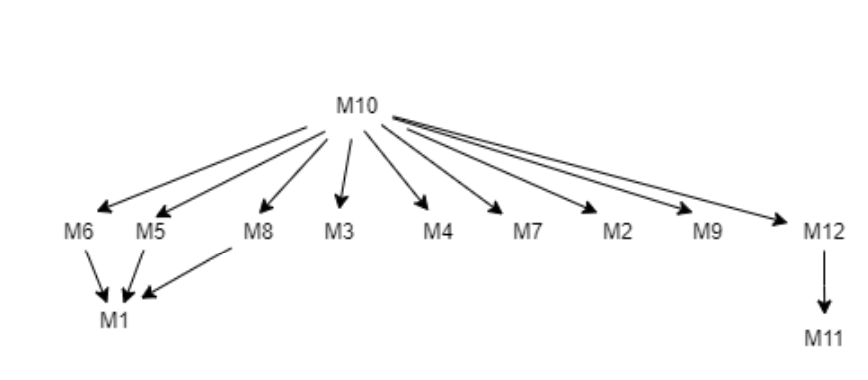
\includegraphics[width=0.7\textwidth]{usesHeirarchy.png}
\caption{Use hierarchy among modules}
\label{FigUH}
\end{figure}

%\section*{References}

\bibliographystyle {plainnat}
\bibliography {MG}

\end{document}
